\documentclass[a4paper]{article}

\usepackage{numprint}
\usepackage{nameref}
\usepackage{float}
\usepackage{url}
\usepackage{graphicx}	% For figure environment
\usepackage{epstopdf}
\usepackage[center]{subfigure}
\usepackage{amssymb}	% For mathematical figures like \mathbb{R}
\usepackage{amsmath}
\usepackage{framed}
\usepackage{tikz}
\usetikzlibrary{mindmap,trees}
\usepackage{pdflscape}
\usepackage[a4paper]{geometry}
\usepackage{subfiles}
\usepackage{listings}
\usepackage{color}

\definecolor{dkgreen}{rgb}{0,0.6,0}
\definecolor{gray}{rgb}{0.5,0.5,0.5}
\usepackage{array}
\usepackage{booktabs}% http://ctan.org/pkg/booktabs
\usepackage{xparse}% http://ctan.org/pkg/xparse
% Rotation: \rot[<angle>][<width>]{<stuff>}
\NewDocumentCommand{\rot}{O{45} O{1em} m}{\makebox[#2][l]{\rotatebox{#1}{#3}}}%
\definecolor{mauve}{rgb}{0.58,0,0.82}

\lstset{frame=tb,
  language=Java,
  aboveskip=3mm,
  belowskip=3mm,
  showstringspaces=false,
  columns=flexible,
  basicstyle={\small\ttfamily},
  numbers=none,
  numberstyle=\tiny\color{gray},
  keywordstyle=\color{blue},
  commentstyle=\color{dkgreen},
  stringstyle=\color{mauve},
  breaklines=true,
  breakatwhitespace=true
  tabsize=3
}


\title{Advanced Systems Lab - Milestone II} 
\author{Lukas Elmer (elmerl@ethz.ch)} 
\date{\today} 


\begin{document}

\maketitle

\pagebreak

\tableofcontents

\pagebreak

\begin{abstract}

This document is the follow up document of Advanced Systems Lab - Milestone I and describes an analytical queueing model of the system which was built using the operational laws. Using this model, the performance characteristics of the model are derived and compared to the measurements of Milestone I. Furthermore it is analysed where the data matches the model and where it does not.

\end{abstract}

\pagebreak

%% ----------------------------------------------
% Section Messaging System
%% ----------------------------------------------
\section{Tasks}

* analytical queuing model
** for each component of the system
** and for the system as a whole.

* derive the performance characteristics that the model predicts
** compare them with the results obtained in milestone 2

* Explain where the model and data match and where they do not match
** sufficiently detailed explanations of characteristics behind the observed behaviour
*** code
*** system
*** hardware

* the modeling should include for each component
** the queuing model(s)
** parameters

* overall system should be modeled
** as queuing network
** the experimental results analyzed using the operational laws

* clearly indicate
** the behavior expected from the model through graphs
** plot them together with the measured behavior

* When evaluating the experimental data and the models
** clearly indicate the laws you are applying
** explain why you think they can be applied in the corresponding analysis



%% ----------------------------------------------
\section{Components}

In the analysis, the focus of the system is on the middleware. Additionally, the database is modelled as a queue, but no further internals of the database are considered.\\

\begin{figure}[H]
	\begin{center}
    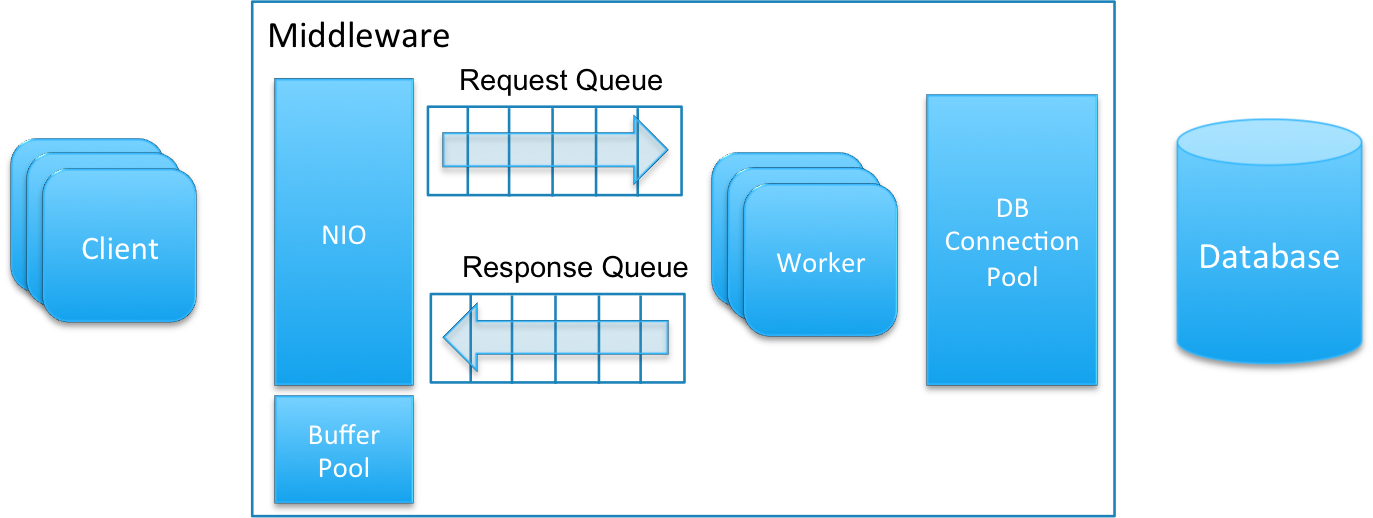
\includegraphics[scale=0.6]{../drawings/broker-threading.png}
  \end{center}
  \caption{Middleware's main Components}
  \label{fig:middleware-threading}
\end{figure}

Figure \ref{fig:middleware-threading} shows a overview of the systems components. The most important parts of the analytical models are:

\begin{itemize}
\item The middleware (multiple instances)
	\begin{itemize}
	\item NIO (network input and output, single queue)
	\item Request queue (when the requests are waiting for workers)
	\end{itemize}
\item The database (modelled as a single queue)
\end{itemize}

Because the clients wait for the current message to be answered before sending the next message, the system is modelled as a \textbf{closed system}. If messages fail to be processed by the middleware, the client implements a backoff time, so the system doesn't get overloaded.

\section{Performance Characteristics}

As described in the book (TODO) in section 30.1, a queuing system can be specified by six parameters. Therefore we use the Kendall notation in the form A/S/m/B/K/SD, where the letters correspond to the six parameters listed on page 507-509 in the book.

\subsection{A: Arrival Process}

Even tough the clients send in a certain deterministic interval, because of the network and the operating system there is a delay until the requests arrive in the queuing system. We assume that this delay is exponentially distributed. Thus, A is the Markovian M. (can be seen in figure TODO)

\subsection{S: Service Time Distribution}

The service time distribution also is assumed to be distributed exponentially. We also know that the service time is memoryless - i.e. it does not matter what request happened before the current request. This can be assumed because there is no caching implemented.

\subsection{m: Number of Servers}

The number of servers is the amount of middlewares running.

\subsection{B: System Capacity}

The system capacity is defined by those who are waiting for service and those who receive service.  This is dependent on how many requests a middleware can accept. Because there are always less clients connected to a middleware then connections to the NIO part of the middlware can be established, the system capacity will be the same as the population size (TODO: check!!!).

\subsection{K: Population Size}

The population size is defined by the amount of clients issuing requests to the middleware.

\subsection{SD: Service Discipline}

In general, the service discipline is First Come, First Served (FCFS). However, because there are limited CPU's on the middleware, and CPU's usually use Round Robin (RR), this may have to be considered in the analysis.


\section{Model}

\subsection{General Model}

The following queueing model network was created based on the understanding of the closed system as shown in figure \ref{fig:general-queueing-network}.

\begin{figure}[H]
	\begin{center}
    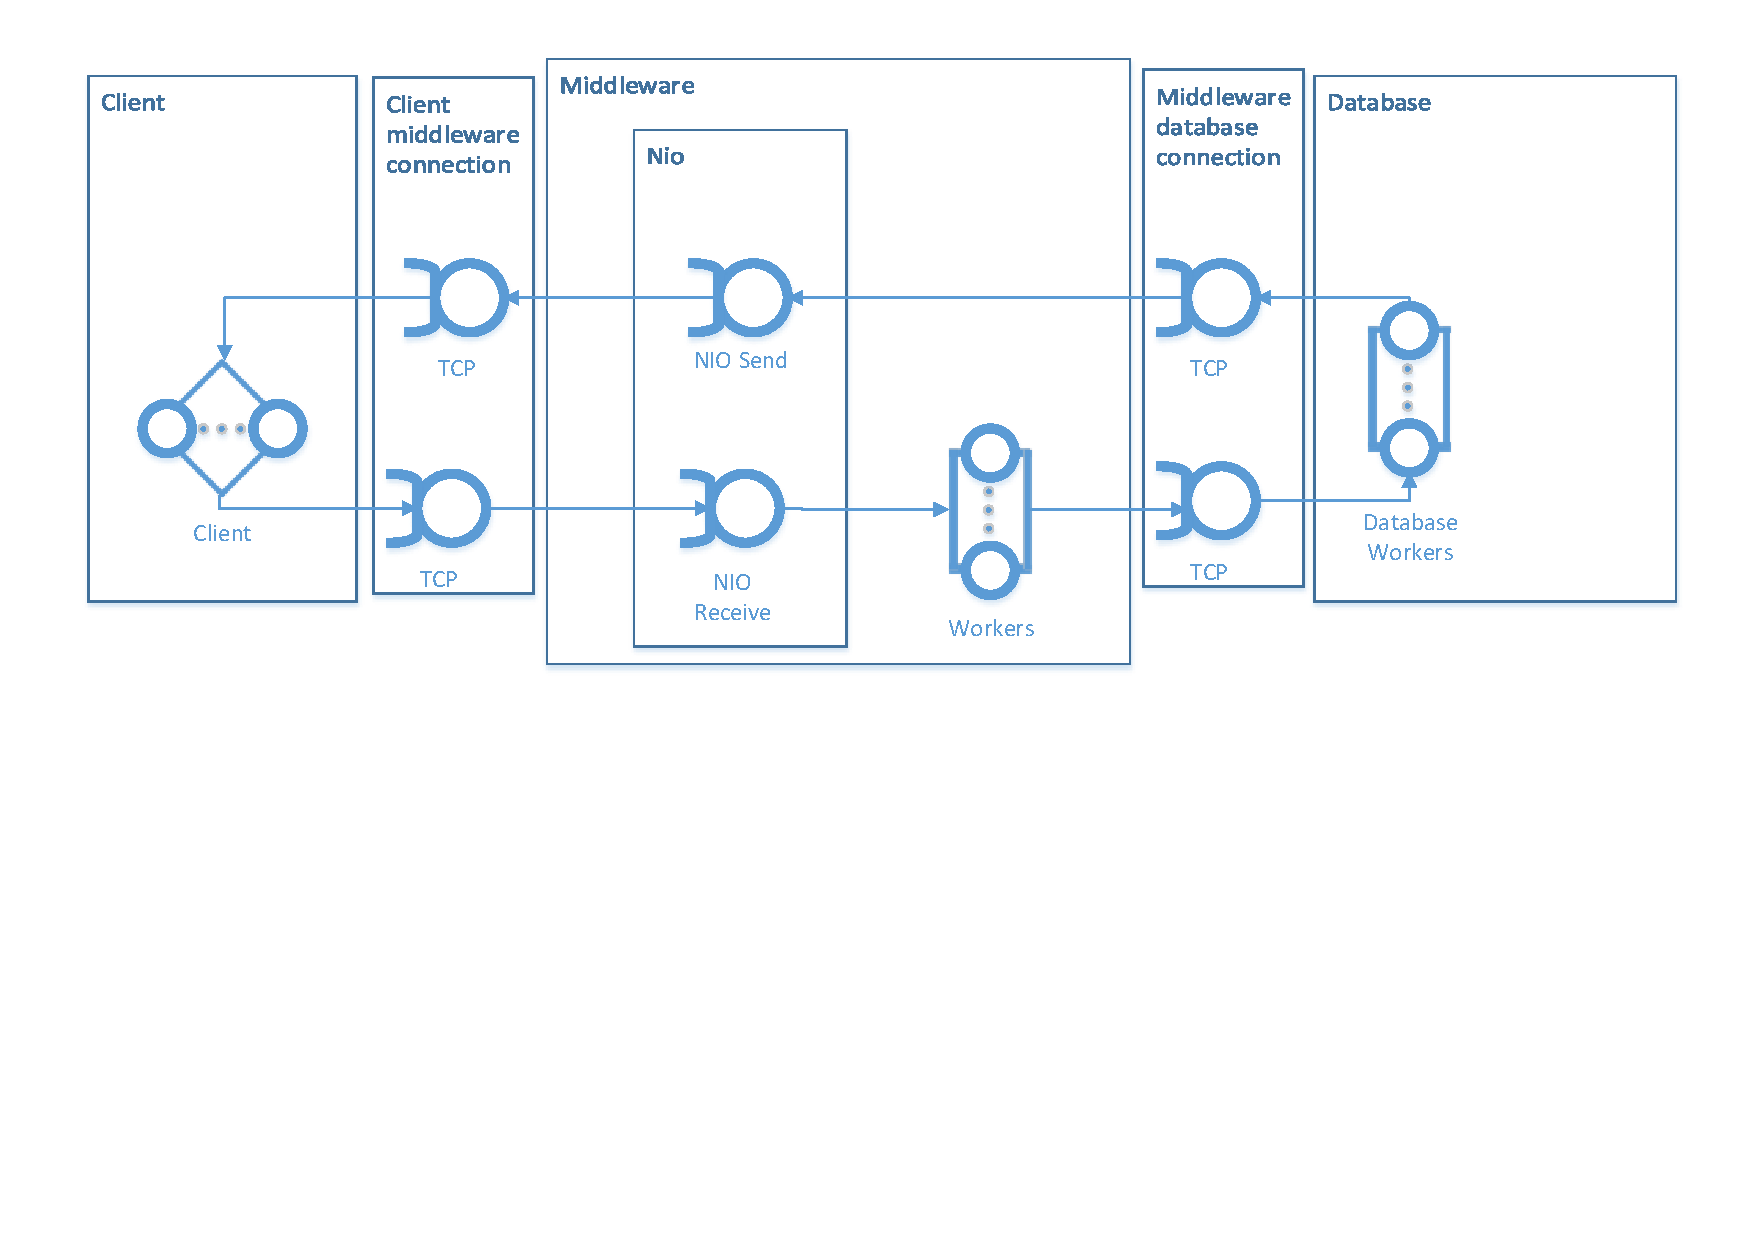
\includegraphics[scale=0.6, trim = 15mm 94mm 12mm 10mm, clip]{../drawings-ms2le/general-queueing-network.pdf}
  \end{center}
  \caption{general queueing network}
  \label{fig:general-queueing-network}
\end{figure}


%Initially the TCP connections were modelled as queues. To simplify the model, the TCP connections were replaced by delay stations.\\

\subsection{Simplified Model}

\noindent Initially the TCP connections are modelled as a separate System. To be precise, these TCP connections would influence one another. In the simplified model, those TCP connections act as separate queues. Additionally, the NIO part of the middleware is included in the TCP connection queue. This is a good idea because the NIO thread and the network are strongly linked and the NIO processing is very fast.\\

\noindent Next, the model was further simplified by separating the NIO component into two separate queues. In the real system however, similar to the TCP connection, there is only one NIO thread.\\

\noindent Furthermore, the TCP network connection between the middleware and the database is separated. In the real system, this would be the same connection.\\

\noindent Those simplifications then lead to the simplified queueing network as shown in figure \ref{fig:simplified-queueing-network}.\\

\begin{figure}[H]
	\begin{center}
    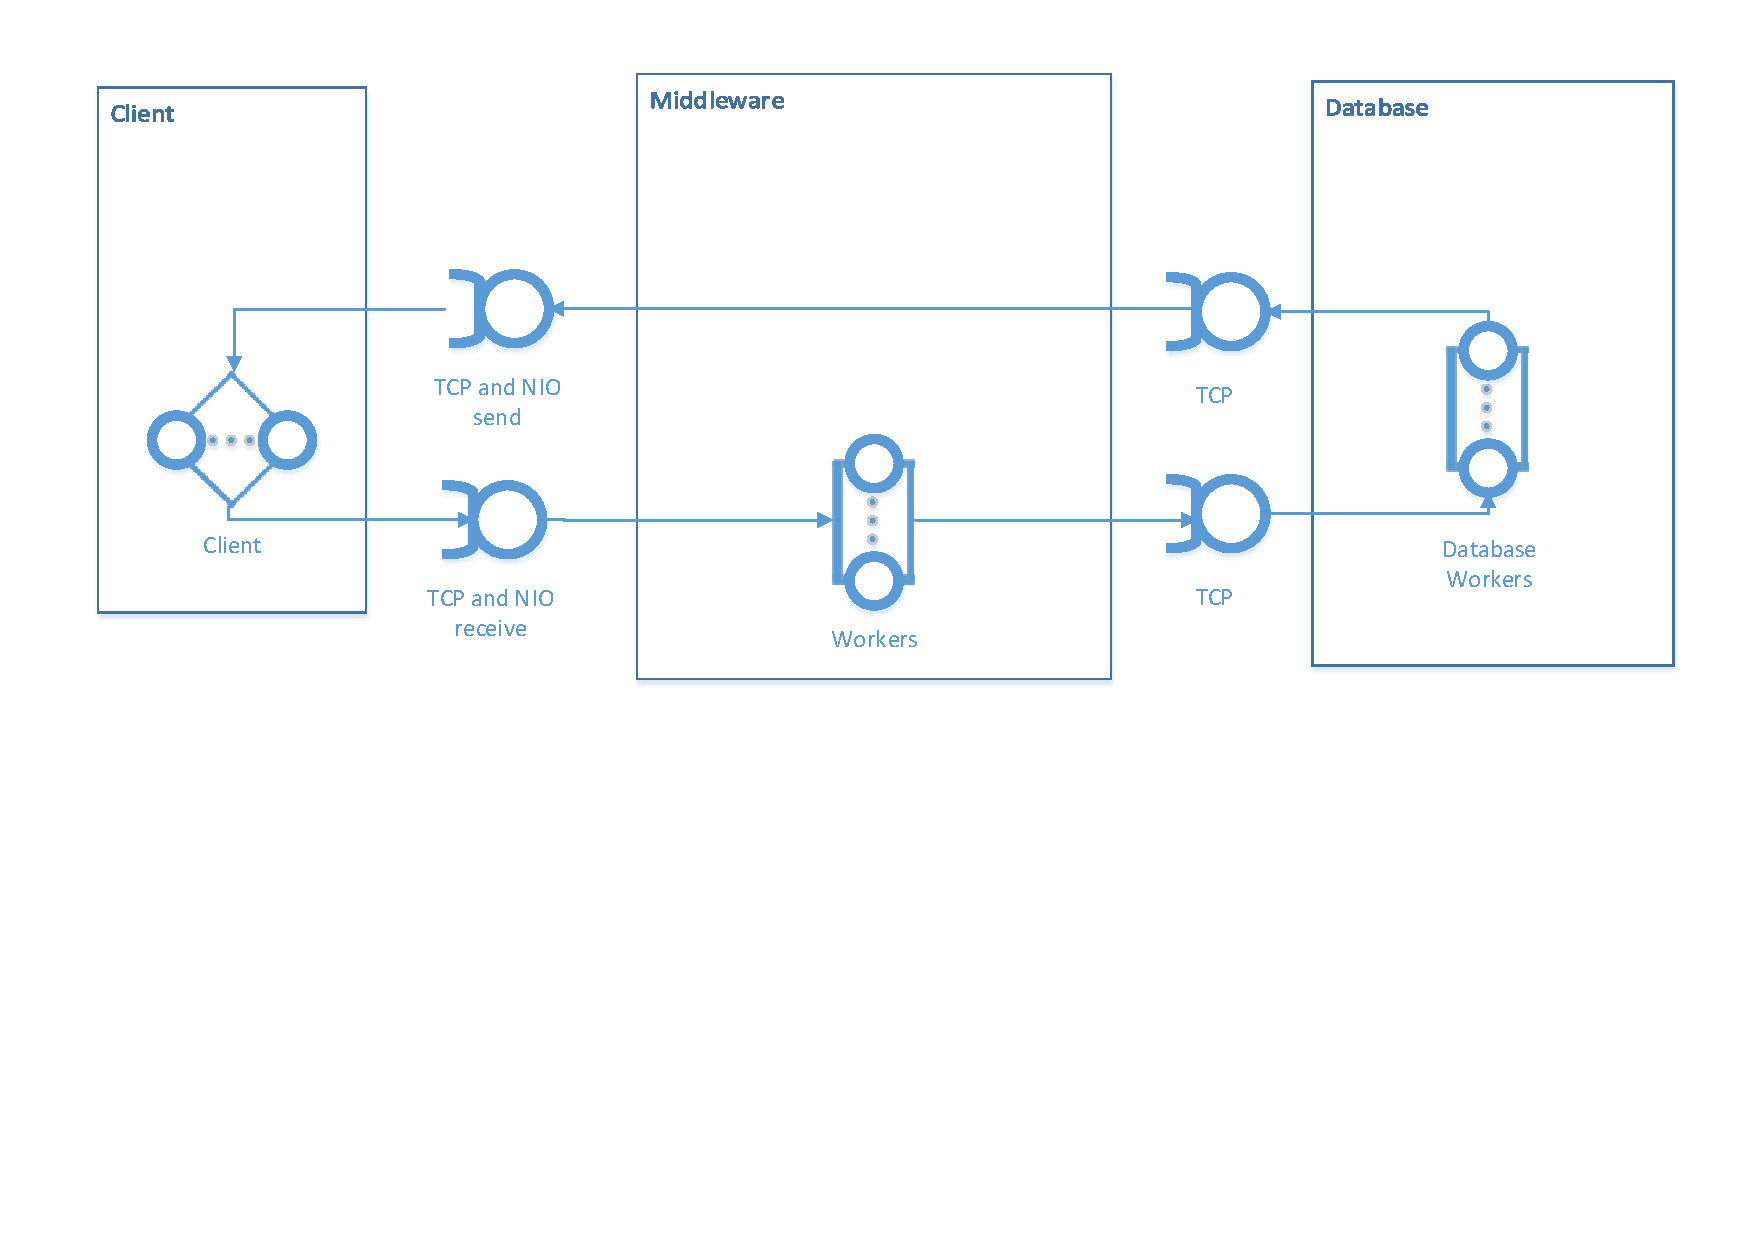
\includegraphics[scale=0.6, trim = 15mm 94mm 12mm 10mm, clip]{../drawings-ms2le/simplified-queueing-network.pdf}
  \end{center}
  \caption{simplified queueing network}
  \label{fig:simplified-queueing-network}
\end{figure}

\subsection{Service Centers}

\subsubsection{Client}

The clients do simple operations (send and receive messages) and don't do any computation. The think time (\textbf{Z}) of the client doesn't depend on the client count and thus correspond to the sleep time between requests.

\subsubsection{TCP and NIO receive / send}

The TCP and NIO receive / send contains many things like the network card, the time it takes to physically transport and rout the signal to the corresponding receiver, the OS buffer, and the JVM network buffer. It was decided to also add the NIO thread to this queue, because it acts like the OS buffer or the JVM network buffer.\\

\noindent The queue is modelled as a fixed capacity service center with and unbound queue size. Because only one network connection and one NIO thread is used, the service node count is 1. So it is modelled as M/M/1 queue.


\subsubsection{Workers (Middleware)}

There are several worker threads in the system. These worker threads are modelled as a M/M/x queue, where x corresponds to the number of worker threads per middleware. The workers obviously are load dependent. The queue size is 100, as it corresponds to the queue size of the queue from which the worker threads can get the requests which have to be processed.\\

\noindent Additionally, the middlewares can be scaled. The clients are evenly distributed between the middlewares, and so are the requests sent by the clients. Therefore, the model is simplified further as follows: for every additional middleware, the workers are merged into one big worker pool across all middlewares. Therefore, the middleware queues are modelled as M/M/(n * x) queues, where n corresponds to the amount of middlewares and x corresponds to the number of worker threads per middleware.\\

\noindent Unfortunately this simplification also means that the "TCP and NIO receive / send" must be changed as a M/M/n queue, where n corresponds to the amount of middlewares. It still can be modelled as an unbound queue.


\subsubsection{TCP}

This is the same as "TCP and NIO receive" without the NIO. Therefore it is also modelled as a fixed capacity service center with unbound queue size and a node count of 1.

\subsubsection{Database}

As stated in the requirements, there must be only one database. However there is never a global table lock and there are multiple ECU's (EC2 Compute Unit\footnote{https://aws.amazon.com/en/ec2/faqs/\#What\_is\_an\_EC2\_Compute\_Unit\_and\_why\_did\_you\_introduce\_it})  available. Furthermore it's unknown how the hardware of the Amazon medium instance is exactly built, but it can be considered that it takes advantage of advanced technology like the locality effect, caching, fail-safe and performance optimized hardware. Unfortunately in one hand, fortunately in the other hand, details about the hardware which the system runs on is unknown. Further information can be found on the amazon website\footnote{https://aws.amazon.com/en/ec2/instance-types/}.\\

Even tough there are 2 ECU's: because there is one vCPU for the medium instance, the node count is set to 1. Also, the service center is modelled as load dependent for obvious reasons.






















\end{document}









